% !TeX root = Documentation-HU.tex

\documentclass[12pt,a4paper,hungarian]{report} 

\usepackage[utf8]{inputenc}
\usepackage[provide=*]{babel}
\usepackage{microtype}
\usepackage{graphicx}

\title{Smart Turntable Assistant}
\author{Daniel Kiss}
\date{\today}

\clubpenalty=100000
\widowpenalty=100000

\begin{document}
\sloppy

\maketitle
\tableofcontents

\chapter{Bevezetés}


Az elmúlt években a zeneipar az analóg fizikai hordozók, különösen a bakelitlemezek népszerűségének példátlan visszatérését tapasztalta. Az audiofileket és a hétköznapi hallgatókat egyaránt vonzza a mechanikus élmény, a szándékos cselekvés, amellyel egy albumot az elejétől a végéig meghallgatnak, valamint az analóg hangzás egyedi, meleg akusztikai jellemzője. Ugyanakkor, egy olyan korszakban, amelyet a digitális streaming platformok, mint a Spotify és az Apple Music uralnak, a hagyományos hanglemez hallgatási élmény alapvetően elszigetelt marad a modern digitális ökoszisztémától.

Ez a szakdolgozat egy Okos Lemezjátszó Asszisztens tervezését, architektúráját és megvalósítását mutatja be, amely egy szoftvervezérelt hidat képez az analóg audio hardverek és a modern digitális kényelmi funkciók között. Valós idejű jelfeldolgozás és külső API integrációk felhasználásával ez a projekt arra törekszik, hogy modernizálja az analóg zenehallgatás élményét anélkül, hogy a bakelit lemez hallgatás élményébe, hangi világába beleszólna.

\section{Problémafelvetés}

Az analóg hangzás alapvető korlátja, hogy egy folyamatos, nyers elektromos jel, amely teljes mértékben nélkülözi a metaadatokat. A digitális hangfájlokkal ellentétben egy lemezjátszó nem képes natív módon tájékoztatni a hallgatót vagy a csatlakoztatott eszközöket arról, hogy éppen mi szól. Ez a technológiai szakadék számos jól elkülöníthető problémát eredményez a modern hanglemez-hallgatók számára:

\begin{enumerate}
    \item \textbf{A digitális integráció hiánya:} A felhasználók nem tudják automatikusan nyomon követni zenehallgatási szokásaikat. A lejátszások naplózása az olyan közösségi zenei platformokra, mint a Last.fm, fárasztó, manuális adatbevitelt igényel.
    \item \textbf{A kontextuális média hiánya:} A modern streaming kényelmi funkciói, mint például a szinkronizált dalszövegek és a nagy felbontású albumborítók megjelenítése, analóg lejátszás közben teljesen elérhetetlenek.
    \item \textbf{Hardveres degradáció nyomon követhetetlensége:} A lemezjátszó tűk élettartama korlátozott, amelynek lejárta után véglegesen károsíthatják a bakelitlemezek barázdáit. A felhasználók jelenleg csak durva becslésekre támaszkodhatnak a hangszedő kopásának nyomon követésében.
    \item \textbf{Hozzáférhető diagnosztika hiánya:} Az olyan problémák azonosítása, mint a túlzott motorrezgés, a felületi sérülések vagy az inner-groove distortion, hagyományosan drága, dedikált akusztikai mérőműszereket igényelnek.
\end{enumerate}

\section{A szakdolgozat célkitűzései}

A szakdolgozat elsődleges célja egy robusztus, valós idejű Kliens-Szerver alkalmazás megtervezése és megvalósítása, amely passzívan figyeli egy szabványos lemezjátszó audio kimenetét, és „okos” funkciók átfogó készletét nyújtja. A rendszert úgy terveztem, hogy egy USB audio interfészhez csatlakoztatott, alacsony erőforrás-igényű hardveren fusson.

A fent vázolt problémák megoldása érdekében a projekt a következő műszaki célkitűzéseket határozza meg:

\begin{itemize}
    \item \textbf{Valós idejű jelfeldolgozás:} Egy konkurens Python backend fejlesztése, amely képes az analóg audio stream folyamatos elemzésére egy zeneszám kezdetének vagy végének detektálásához, valamint a hardverdiagnosztikai adatok matematikai kiszámításához.
    \item \textbf{Audio Fingerprinting és metaadat-bővítés:} Egy robusztus felismerési pipeline implementálása, amely rövid hangmintákat rögzít, és audio fingerprinting szolgáltatások segítségével azonosítja azokat. Továbbá egy waterfall elvű metaadat-lekérdező rendszer tervezése, amely megbízhatóan lekéri a pontos sávhosszakat, albumneveket és nagy felbontású borítóképeket.
    \item \textbf{Automatizált digitális szinkronizáció:} Háttérszolgáltatások létrehozása az időbélyeggel ellátott dalszövegek letöltésére, valamint egy automatizált Last.fm scrobbling funkció implementálása, amely pontosan tiszteletben tartja a sáv eltelt lejátszási idejét.
    \item \textbf{Adatbázis- és hardverkezelés:} Egy relációs adatbázis megvalósítása a hallgatási előzmények tárolására, a testreszabott vizuális preferenciák mentésére, valamint a felhasználó által definiált lemezjátszó-hangszedők életciklusának pontos nyomon követésére.
    \item \textbf{Modern, reaktív felhasználói felület:} Egy reszponzív Single Page Application (SPA) tervezése Vue.js használatával, amely WebSockets technológián keresztül kommunikál a backenddel. Az interfésznek zero-latency vizuális visszajelzést kell nyújtania a felhasználók számára, és dinamikus tematikus testreszabhatóságot kell kínálnia.
\end{itemize}

\chapter{Technológiai háttér és szakirodalmi áttekintés}

Egy valós idejű hardvermonitorozó és zenefelismerő rendszer fejlesztése számos tudományág integrációját igényli, a digitális jelfeldolgozástól a modern webalkalmazás-architektúrákig. Ez a fejezet áttekinti azokat az alapvető technológiákat, algoritmusokat és keretrendszereket, amelyeket a projekt megvalósításához választottam.

\section{Audio Fingerprinting technológiák}

Az audio fingerprinting egy olyan mechanizmus, amelyet egy hangminta azonosítására használnak egyedi akusztikai jellemzők kinyerésével és azok egy ismert adatbázissal történő összehasonlításával. Az alapvető metaadat-címkézéssel ellentétben a fingerprinting a tényleges audiotartalmat elemzi. A folyamat jellemzően az audiojel spektrogrammá alakítását, a nagy energiájú pontok vagy csúcsok azonosítását, és egy constellation map létrehozását foglalja magában. Ezeket a csúcsokat ezután kompakt digitális aláírásokká alakítják.

Ez a matematikai megközelítés rendkívül ellenálló a háttérzajjal, a hangmagasság-torzulással és a bakelitlemezekre jellemző felületi sercegéssel szemben. Ebben a projektben iparági szabványnak számító felismerő motorokat – köztük a Shazam API-t és az ACRCloud-ot – alkalmazok a fingerprint egyeztetés elvégzésére. Ezek a szolgáltatások a rögzített audio buffereket hatalmas kereskedelmi adatbázisokkal vetik össze, hogy az analóg tökéletlenségek ellenére is pontosan azonosítsák a lejátszott sávot.

\section{Alkalmazott keretrendszerek}

Az alkalmazás architektúrája a felelősségi körök szigorú szétválasztásán alapul, egy robusztus backend-re és egy dinamikus frontend-re osztva.

A backend esetében a választás a Pythonra esett, a matematikai számításokhoz és a digitális jelfeldolgozáshoz rendelkezésre álló kiterjedt ökoszisztémája miatt. Az olyan könyvtárak, mint a NumPy és a SciPy, kulcsfontosságúak a tömbműveletek elvégzésében, a frekvenciaszűrésben és az akusztikai metrikák valós idejű kiszámításában. A webszerver réteget a Flask hajtja meg. Lightweight mikro-keretrendszerként a Flask biztosítja a szükséges eszközöket egy RESTful API kiajánlásához és az adatbázis-munkamenetek kezeléséhez a SQLAlchemy ORM-en keresztül, felesleges overhead bevezetése nélkül.

A frontend egy Vue.js alapú Single Page Application-ként került implementálásra. A Vue a reaktív, komponens-alapú architektúrája miatt bizonyult ideális választásnak, amely lehetővé teszi, hogy a felhasználói felület azonnal frissüljön a mögöttes adatok változásakor. A globális állapotkezelést a Pinia végzi, biztosítva, hogy a hardverbeállítások, a felhasználói hitelesítési állapotok és az aktuális lejátszási metaadatok tökéletesen szinkronizálva maradjanak az alkalmazás összes nézetében.

\section{Valós idejű kommunikáció}

A rendszer egyik alapvető követelménye, hogy a hardverdiagnosztikát és a szinkronizált dalszövegeket érzékelhető késleltetés nélkül jelenítse meg. A hagyományos HTTP polling, ahol a kliens ismétlődően kér adatokat a szervertől, jelentős hálózati többletterhelést okoz, és teljesen alkalmatlan a nagyfrekvenciás audio vizualizációra.

Ennek megoldására az alkalmazás WebSockets technológiát alkalmaz. A WebSockets folyamatos, full-duplex kommunikációs csatornát hoz létre egyetlen TCP kapcsolaton keresztül. Ez lehetővé teszi a Python backend számára, hogy folyamatosan adatokat toljon kifelé anélkül, hogy megvárná a kliens kérését. A Socket.IO könyvtár hidat képez a Flask backend és a Vue frontend között, elősegítve a hangerőszintek, a click detection események és a lejátszási időzítők zökkenőmentes sugárzását, másodpercenként tíz képkockás sebességgel.

\section{Fejlesztési és futtatási környezet}

Annak biztosítása, hogy a szoftver megbízhatóan fusson a különböző operációs rendszereken, szigorú környezeti izolációt igényel. A konténerizációhoz a Docker került felhasználásra, amely a teljes alkalmazást és a rendszerszintű függőségeit szabványosított egységekbe csomagolja.

Az audio alkalmazások konténerizálásának jelentős kihívása, hogy az izolált környezet számára hozzáférést kell biztosítani a host hardveréhez. Ezt a problémát a gazdagép hangeszközeinek a Docker konténerbe történő leképezésével, valamint az Advanced Linux Sound Architecture (ALSA) és a PulseAudio alrendszerek áthidalásával oldottam meg. Ez a beállítás lehetővé teszi, hogy az alkalmazás fejlesztés közben zökkenőmentesen telepíthető legyen szabványos asztali számítógépekre, miközben tökéletesen optimalizált marad a végső production environment, például egy alacsony fogyasztású, egykártyás számítógépre, mint a Raspberry Pi.

\chapter{Követelményanalízis}

Az architekturális tervezés és a szoftverimplementációs fázisok előtt a rendszerkövetelmények átfogó elemzése szükséges. Ez biztosítja, hogy a végtermék sikeresen áthidalja az analóg hanglemez-lejátszás és a modern digitális kényelmi funkciók közötti szakadékot. Ez a fejezet felvázolja a rendszer elvárt specifikus funkcionális képességeit, azokat a nem-funkcionális minőségi attribútumokat, amelyeknek meg kell felelnie, valamint a felhasználói interakciót meghatározó elsődleges használati eseteket.

\section{Funkcionális követelmények}

A funkcionális követelmények határozzák meg azokat a pontos viselkedéseket, folyamatokat és funkciókat, amelyeket a Smart Turntable Assistant-nek végre kell hajtania, hogy értéket teremtsen a végfelhasználó számára.

\begin{itemize}
    \item \textbf{Valós idejű audio azonosítás:} A rendszernek folyamatosan figyelnie kell a bejövő audio streamet, és automatikusan detektálnia kell a lejátszás kezdetét. Az észlelés után rögzítenie kell egy rövid audio buffert, és külső audio fingerprinting API-kat kell lekérdeznie a sáv azonosításához.
    \item \textbf{Metaadat-bővítés:} Sikeres audio egyeztetés után az alkalmazásnak másodlagos zenei adatbázisokat kell lekérdeznie. Ez a lépés szükséges a nagy felbontású albumborítók, a pontos sávhosszúság (milliszekundumban), és a szabványosított albumnév lekéréséhez.
    \item \textbf{Szinkronizált dalszöveg megjelenítés:} A backendnek le kell töltenie az időbélyeggel ellátott dalszövegfájlokat az azonosított zeneszámhoz. A frontendnek értelmeznie kell ezeket az időbélyegeket, és automatikusan kell görgetnie a szöveget, szinkronban az élő lejátszási időzítővel. A felhasználónak lehetőséget kell biztosítani a szinkronizációs idővonal manuális eltolására az apró mechanikai késleltetések korrigálása érdekében.
    \item \textbf{Hardverállapot-diagnosztika:} A szoftvernek elemeznie kell a bejövő analóg jelet az effektív (RMS) hangerőszint kiszámításához. Matematikailag fel kell dolgoznia a hangot a hirtelen felületi kattogások detektálására, az alacsony frekvenciás mechanikai motorrezgés mérésére, és a magas frekvenciás sziszegő torzítás (sibilance) számszerűsítésére.
    \item \textbf{Hangszedő életciklus kezelés:} A rendszernek fenn kell tartania egy adatbázist a felhasználó tulajdonában lévő lemezjátszó tűkről. Nyomon kell követnie az éppen aktív hardver kumulatív lejátszási idejét, lehetővé kell tennie a felhasználó számára a maximálisan ajánlott élettartam meghatározását, és biztosítania kell a számláló nullázásának lehetőségét a hardver cseréjekor.
    \item \textbf{Digitális hallgatási naplók:} Az alkalmazásnak támogatnia kell a hitelesítést külső, közösségi zene-nyomonkövető szolgáltatásokkal, mint amilyen a Last.fm. Automatikusan naplóznia kell a zeneszámot a felhasználó profiljába, amint a lejátszás eléri a meghatározott időtartam-küszöböt.
    \item \textbf{Esztétikai testreszabás:} A webes felületnek lehetővé kell tennie a felhasználók számára, hogy testreszabják a digitális lemez vizuális megjelenését a színes fizikai hordozóknak megfelelően. Ezt a színpreferenciát az adatbázisba kell menteni, és automatikusan újra kell alkalmazni, valahányszor az adott albumról szóló zeneszám lejátszásra kerül.
\end{itemize}

\section{Nem-funkcionális követelmények}

A nem-funkcionális követelmények diktálják azokat a teljesítményszabványokat, megbízhatósági korlátokat és használhatósági metrikákat, amelyeket a rendszerarchitektúrának ki kell elégítenie.

\begin{itemize}
    \item \textbf{Teljesítmény és késleltetés:} A háttérben futó audiofeldolgozó szálnak folyamatosan működnie kell anélkül, hogy blokkolná a webszerver műveleteit. A diagnosztikai adatokat másodpercenként többször kell a frontend felé sugározni a folyékony vizuális animációk és a pontos VU Meter-ek, hangszint jelzők.
    \item \textbf{Megbízhatóság és Fallback mechanizmusok:} A külső adatbázisok felé irányuló hálózati lekérdezéseknek robusztus fallback stratégiákat kell alkalmazniuk. Ha egy elsődleges felismerő motor vagy metaadat-szolgáltatás meghibásodik, a rendszernek zökkenőmentesen meg kell próbálnia a másodlagos források használatát az adatvesztés elkerülése és a folyamatos működés biztosítása érdekében.
    \item \textbf{Használhatóság és reszponzivitás:} A grafikus felhasználói felületnek dinamikusan kell skálázódnia a különböző kijelzőméretek között, a mobiltelefonok képernyőitől a nagy felbontású asztali monitorokig. Konténer-lekérdezéseket és folyékony tipográfiát kell alkalmazni az elrendezés integritásának megőrzéséhez.
    \item \textbf{Adatbázis-konkurencia:} A mögöttes relációs adatbázisnak támogatnia kell az egyidejű olvasási és írásási műveleteket. A háttérszálaknak képesnek kell lenniük a hangszedő statisztikáinak frissítésére, miközben az azonosító szál egyidejűleg új hallgatási előzményeket ment, amely az adatbázis-zárolási hibák megelőzése érdekében Write-Ahead Logging módot igényel.
\end{itemize}

\section{Használati esetek}

A következő használati esetek a hallgató és a Smart Turntable Assistant közötti elsődleges interakciókat szemléltetik egy tipikus zenehallgatási munkamenet során.

\begin{itemize}
    \item \textbf{Automatizált lejátszás-monitorozás:} A felhasználó ráengedi a tűt egy bakelitlemezre. A rendszer detektálja az audio küszöbértéket, azonosítja a számot, és automatikusan, manuális beavatkozás nélkül feltölti a dashboardot a megfelelő albumborítóval és a szinkronizált dalszöveggel.
    \item \textbf{Hardverdiagnosztika megfigyelése:} A felhasználó a diagnosztika fülre navigál, miközben egy lemez szól. Figyeli az élő felületet, hogy ellenőrizze a lemezjátszó motorjának megfelelő szigetelését, és figyeli a click counter-t annak megállapítására, hogy a bakelit felülete tisztítást igényel-e.
    \item \textbf{Hangszedő konfigurációja:} A felhasználó megnyitja személyes profilját egy újonnan vásárolt tű regisztrálásához. A gyártó ajánlásai alapján beállítja a várható élettartamot, aktív hardverként jelöli meg, majd visszatér a dashboardra, hogy figyelemmel kísérje a hátralévő élettartam százalékos arányát.
    \item \textbf{Vizuális felület testreszabása:} Miközben a felhasználó egy album áttetsző piros bakelit kiadását hallgatja, a digitális vizualizálóval interakcióba lépve megváltoztatja a megjelenítési stílust, hogy az illeszkedjen a fizikai hordozóhoz. A rendszer ezt a preferenciát a memóriába menti, és automatikusan alkalmazza ugyanezt a vizuális stílust, amikor a jövőben ebből az albumból származó szám kerül lejátszásra.
\end{itemize}

\begin{figure}[htbp]
    \centering
    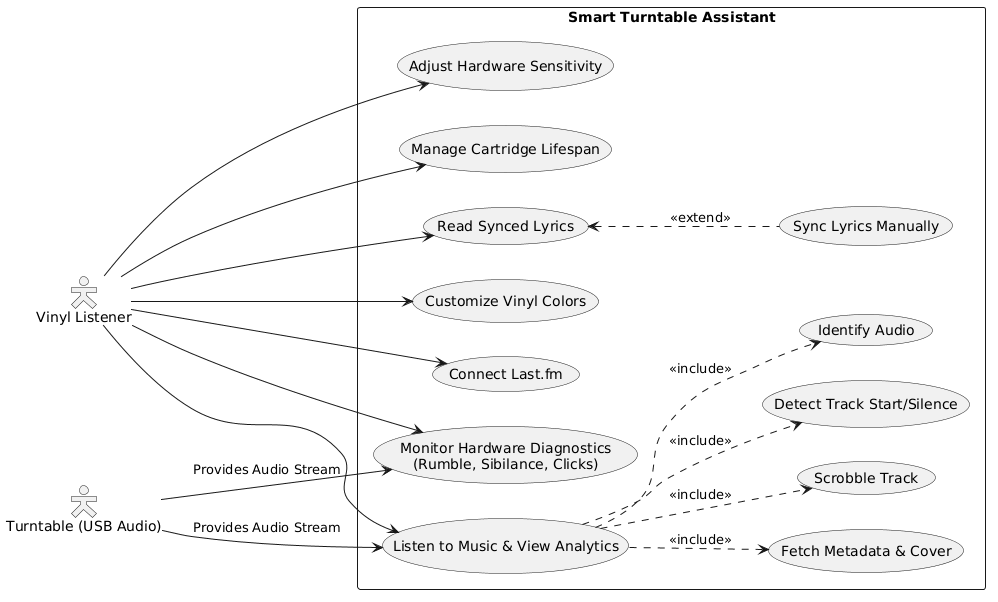
\includegraphics[width=0.8\textwidth]{Images/usecase.png}
    \caption{UML Use Case Diagram illustrating user and system interactions.}
    \label{fig:usecase}
\end{figure}

\chapter{Rendszerterv és architektúra}

Egy folyamatos analóg audiojel strukturált, interaktív digitális élménnyé alakítása erősen szétválasztott és konkurens rendszerarchitektúrát igényel. Ez a fejezet a Smart Turntable Assistant szerkezeti felépítését részletezi, felvázolva a kliens-szerver kommunikációs protokollokat, a relációs adatbázis sémáját, valamint azt az összetett szálkezelést, amely a valós idejű telemetria és az aszinkron hálózati kérések egyidejű feldolgozásához szükséges.

\section{Kliens-Szerver architektúra}

Az alkalmazás architektúrája egy robusztus kliens-szerver modellt követ, amelyet mind a perzisztens adatműveletek, mind a nagyfrekvenciás valós idejű telemetria kezelésére terveztek. A backendet a Python és a Flask mikro-keretrendszer hajtja meg, amely központi feldolgozó egységként működik, és az Advanced Linux Sound Architecture (ALSA) valamint a PulseAudio alrendszereken keresztül közvetlenül kapcsolódik a host audio hardveréhez.


A frontend egy Vue.js keretrendszerrel épített Single Page Application (SPA), amely interaktív dashboardként szolgál a felhasználó számára. A kommunikáció e két eltérő környezet között kétirányú. A szabványos állapotváltozásokat – mint például a felhasználói hitelesítés, a hardveres konfigurációk frissítése és a manuális szinkronizációs beállítások – állapotmentes REST (Representational State Transfer) API végpontok kezelik.

Ezzel szemben az audiodiagnosztika és a lejátszási időzítők folyamatos áramlása állandó, alacsony késleltetésű kapcsolatot tesz szükségessé. Ezt WebSockets technológiával, a Socket.IO könyvtár segítségével értük el. Egy full-duplex kommunikációs csatorna kiépítésével a backend másodpercenként többször képes a hangerőre, a rumble-re és a sibilance-re vonatkozó matematikai számításokat a frontend felé tolni, biztosítva, hogy a felhasználói felület rendkívül reszponzív maradjon, és tökéletes szinkronban legyen a fizikai lemezjátszóval.

\begin{figure}[htbp]
    \centering
    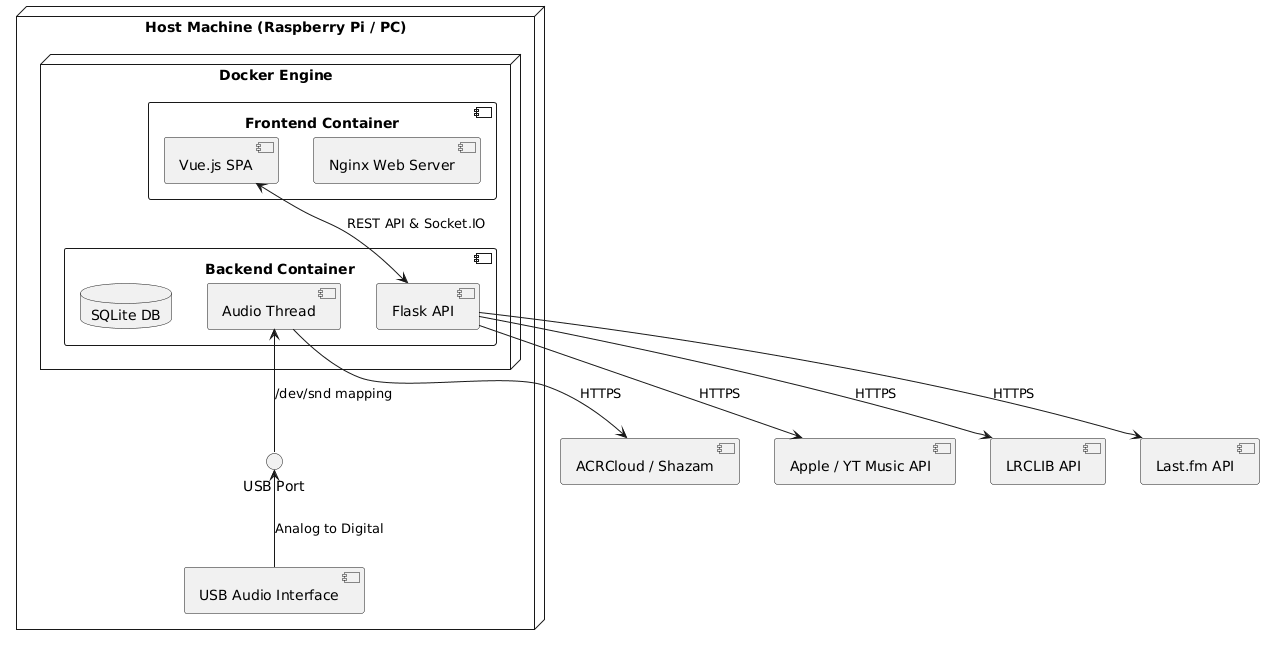
\includegraphics[width=1\textwidth]{Images/deployement.png}
    \caption{Deployment diagram amely a docker image felépítését mutatja be.}
    \label{fig:deployment}
\end{figure}

\section{Adatbázis-tervezés}

A perzisztens adattárolást egy relációs adatbáziskezelő rendszer, konkrétan az SQLite kezeli, a SQLAlchemy ORM (Object-Relational Mapper) integrálásával. A séma normalizált, így a felhasználói hitelesítő adatok, a hardveres metrikák és a historikus zenehallgatási szokások biztonságosan elkülönülnek.

A séma magjában a \texttt{User} (felhasználó) entitás áll, amely egy-a-többhöz kapcsolatot tart fenn az összes többi táblával, biztosítva az adatok izolációját egy többfelhasználós környezetben. A \texttt{Cartridge} (Hangszedő) tábla a felhasználó tulajdonában lévő fizikai lemezjátszó tűket követi nyomon, tárolva azok maximálisan ajánlott élettartamát, valamint a lemezjátszón aktívan eltöltött, kumulatív üzemórákat.

A \texttt{TrackHistory} tábla digitális hallgatási naplóként funkcionál, amely minden egyes sikeres audio felismerési eseménynél rögzíti az azonosított előadót, az albumot és a nagy felbontású borítókép URL-jét (Uniform Resource Locator). Az alkalmazás esztétikai és szinkronizációs funkcióinak támogatása érdekében az \texttt{AlbumColor} és a \texttt{TrackOffset} táblák a felhasználó által meghatározott vizuális preferenciákat és a dalszöveg-időzítési kalibrációkat tárolják, kifejezetten az azonosított előadóhoz és albumhoz kapcsolva azokat. Ez a relációs struktúra biztosítja, hogy amikor a felhasználó bejelentkezik, az aktív tű limiteit és a korábbi zeneszám-módosításait a rendszer azonnal lekérje, és alkalmazza a globális alkalmazás-állapotra.

\begin{figure}[htbp]
    \centering
    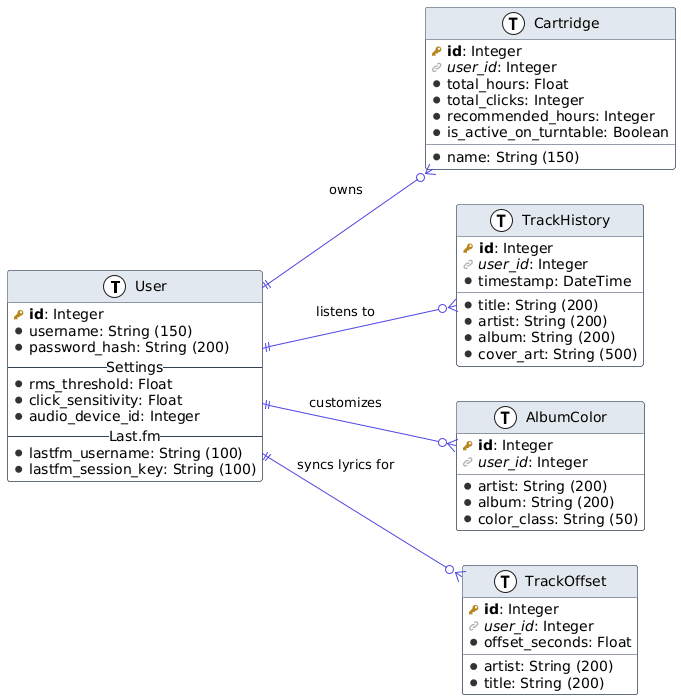
\includegraphics[width=0.85\textwidth]{Images/database.png}
    \caption{Entity-Relationship Diagram az adatbázis sémáról.}
    \label{fig:database}
\end{figure}

\section{Konkurencia és szálkezelés}

Az élő audio streamek elemzése és a külső webszolgáltatások egyidejű lekérdezése jelentős konkurencia-kihívást jelent. Egy tisztán szinkron megközelítés azt eredményezné, hogy az alkalmazás blokkolná az összes diagnosztikai számítást, és lefagyasztaná a felhasználói felületet, amíg egy audio fingerprinting szolgáltatás hálózati válaszára vár. Ennek megoldására a backend egy többszálú architektúrát alkalmaz, amelyet egy centralizált globális állapot-objektum köré szerveztek.

Az elsődleges audiofeldolgozó szál folyamatosan fut a háttérben. Különálló blokkokban olvassa be a hangot a hardveres pufferből, kiszámítja az RMS (Root Mean Square) értékeket, detektálja a felületi kattogásokat (clicks), és frissíti az aktív hangszedő használati statisztikáit. Amikor ez az elsődleges szál a kitartott hangerő-küszöbértékek alapján matematikailag megállapítja, hogy egy új dal kezdődött, elindít egy független, párhuzamos azonosító szálat.

Ez a másodlagos szál rögzít egy ideiglenes hangmintát, és kezeli a fingerprinting motorok, valamint a metaadat-bővítő API-k felé irányuló, késleltetett hálózati kéréseket. Mivel több szál lép egyszerre interakcióba az adatbázissal, az SQLite adatbázis Write-Ahead Logging (WAL) módra van konfigurálva. Ez a fejlett konkurencia-mód lehetővé teszi, hogy az elsődleges szál biztonságosan mentse a hangszedő kopási statisztikáit a lemezre, miközben a másodlagos azonosító szál aktívan írja az új hallgatási előzmény-rekordokat, ezáltal teljesen kiküszöbölve az adatbázis-zárolási hibákat, és biztosítva a zökkenőmentes háttérműködést.

\begin{figure}[htbp]
    \centering
    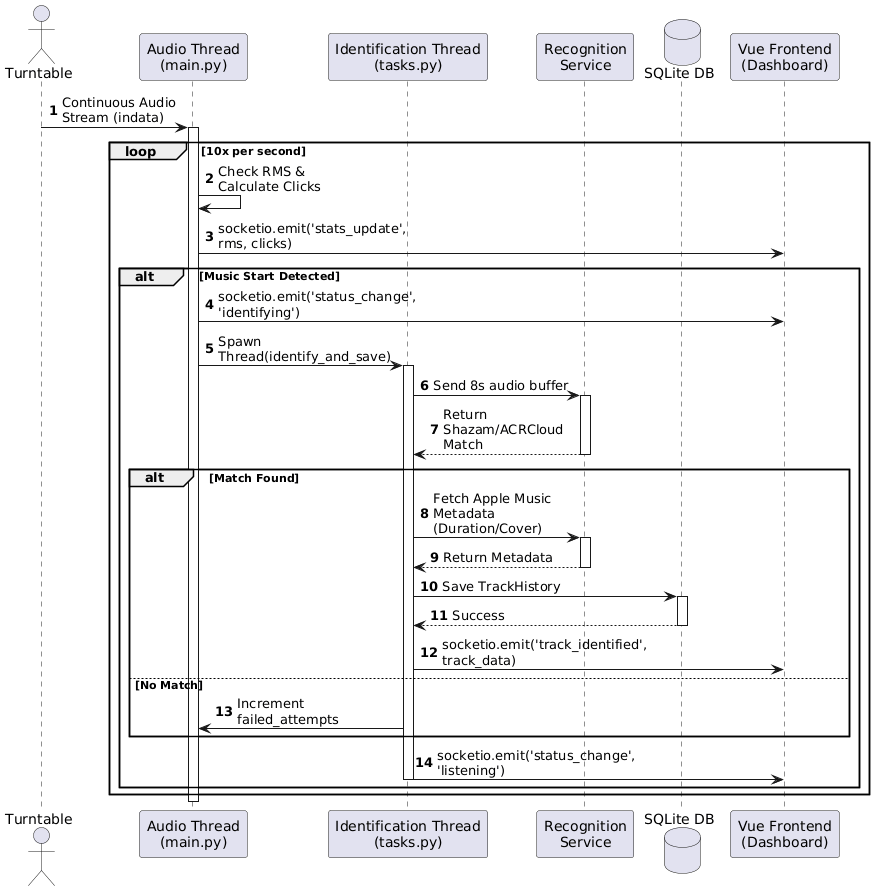
\includegraphics[width=1\textwidth]{Images/sequence.png}
    \caption{UML Sequence Diagram a többszálú kezelésről.}
    \label{fig:sequence}
\end{figure}

\chapter{Megvalósítási részletek}

Az architekturális terv funkcionális alkalmazássá alakítása precíz programozási módszertanokat, robusztus hibakezelést és hatékony algoritmustervezést igényel. Ez a fejezet a Smart Turntable Assistant konkrét implementációját részletezi, feltárva a digitális jelfeldolgozás (DSP) matematikáját, a lépcsőzetes metaadat-lekérdező logikát és a reaktív frontend renderelési technikákat.

\section{Digitális jelfeldolgozás (Digital Signal Processing)}

Az alkalmazás magja a lemezjátszó által biztosított analóg audiojel folyamatos elemzésén alapul. A Python backend a \texttt{sounddevice} és a \texttt{NumPy} könyvtárak felhasználásával, diszkrét matematikai tömbökben rögzíti a hangot. Ezeket az adatblokkokat a rendszer másodpercenként többször feldolgozza a jelentéssel bíró diagnosztikai metrikák kinyerése érdekében.

Annak detektálására, hogy a felhasználó mikor teszi rá a tűt a lemezre, a rendszer kiszámítja az audio chunk RMS értékét, amely az átlagos akusztikus energiát reprezentálja. Ha ez az energia egy megadott ideig a felhasználó által definiált küszöbérték felett marad, az alkalmazás regisztrál egy "lejátszás kezdete" (playback start) eseményt.

A felületi tökéletlenségek, mint a por és a karcolások, hirtelen, magas frekvenciájú tranziensekként jelennek meg, amelyeket kattogásnak vagy sercegésnek (clicks or pops) nevezünk. A szoftver ezeket úgy detektálja, hogy kiszámítja az audiojel első deriváltját, amely felüláteresztő szűrőként (high-pass filter) funkcionál a gyors változások izolálására. Ezen változások szórásának kiszámításával az algoritmus azonosítja azokat a statisztikai kiugró értékeket, amelyek meghaladnak egy adott érzékenységi szorzót, sikeresen megszámolva ezáltal a diszkrét felületi zajokat.

A fejlettebb diagnosztikák közé tartozik a mechanikai motorzaj (rumble) és a sziszegés (sibilance) nyomon követése. A rumble kiszámításához az alkalmazás Fast Fourier Transzformációt (FFT) alkalmaz az audio tömbön, elszigetelve és összegezve a kizárólag tíz Hertz és ötven Hertz közötti akusztikus energiát. A sibilance-t, amely a magas frekvenciájú követési torzítást (tracking distortion) jelzi, úgy méri, hogy a jelet átvezeti egy Butterworth sávszűrőn (bandpass filter), amely az öt kilohertztől tíz kilohertzig terjedő tartományt célozza meg. Ennek az izolált sávnak az energiáját arányosítja a teljes jelenergiával, ami egy olyan százalékos értéket ad eredményül, amely dinamikusan vezérli a frontend felületén lévő "harshness", torzítás mérőt.

\section{A vízesés elvű metaadat-stratégia}

Ha a zenefelismerést és a metaadatokat kizárólag egyetlen külső szolgáltatásra bízzuk, az gyakran hiányos információkat eredményez, különösen az underground vagy rétegzenei műfajok esetében. Ennek megoldására az alkalmazás egy cascading waterfall stratégiát alkalmaz, amely szigorú prioritási sorrendben kérdez le több API-t.

A folyamat egy nyolcmásodperces hangminta rögzítésével kezdődik, amelyet a rendszer aszinkron módon elküld az audio fingerprinting motoroknak. Ha találatot regisztrál, a rendszer kinyeri a payload-ba (válaszadathalmazba) ágyazott egyedi Apple Music azonosítót. Ez a specifikus azonosító lehetővé teszi a backend számára, hogy közvetlenül lekérdezze az iTunes webszolgáltatást, garantálva a pontos sávhossz (milliszekundumban), a hivatalos albumnév és egy nagy felbontású, négyzet alakú albumborító sikeres letöltését.

Ha az elsődleges fingerprinting szolgáltatás nem biztosít pontos azonosítót, a rendszer visszalép egy szövegalapú keresésre a \texttt{ytmusicapi} könyvtár segítségével. Ez a könyvtár a hivatalos YouTube Music katalógust olvassa le. Annak érdekében, hogy a frontend nagy felbontású grafikát kapjon az alacsony felbontású videó indexképek helyett, a szoftver manipulálja a dinamikusan generált kép URL-jét: lecseréli az alapértelmezett dimenzió-paramétereket szigorú, nagy felbontású kérésekre, így tökéletesen éles képeket biztosítva a felhasználói felület számára.

\section{Backend állapotkezelés és adat-streamelés}

Az adatáramlás kezelése a párhuzamos háttérszálak és a csatlakoztatott webes kliensek között egy központosított igazságforrást, úgynevezett source of truth-t igényel. A backend egy globális állapot objektumot valósít meg, amely tartalmazza az aktuális zeneszám metaadatait, az élő diagnosztikai értékeket és a lejátszási időzítőket.

Mivel az audiofeldolgozó szál másodpercenként tízszer értékeli ki az adatokat, a hangszedő-használati statisztikák közvetlenül az SQLite adatbázisba történő írása ilyen gyakorisággal súlyos I/O szűk keresztmetszeteket okozna, és rontaná a tárolóeszköz élettartamát. Ehelyett a rendszer az eltelt lejátszási másodperceket és a kattogások számát ideiglenes memóriaváltozókban halmozza fel. Egy szabályozó mechanizmus gondoskodik arról, hogy ezek a felhalmozott értékek csak tíz másodpercenként kerüljenek elmentésre a fizikai adatbázisba. Ezzel egyidejűleg az élő értékeket a Socket.IO kapcsolaton keresztül a rendszer kisugározza az összes csatlakoztatott kliens felé, biztosítva, hogy a frontend folyékony, valós idejű animációkat jelenítsen meg anélkül, hogy túlterhelné a szerver hardverét.

\section{Frontend interfész és reaktív architektúra}

A felhasználói felületet egy Single Page Application-ként (SPA) terveztük meg a Vue.js keretrendszer használatával, azzal a céllal, hogy függetlenítse a vizuális megjelenítést a backend logikától.

\subsection{Kliens állapot és Útválasztás}
A globális kliens állapotot – beleértve a felhasználói hitelesítést és a session tokeneket – a Pinia állapotkezelő könyvtár (state management library) kezeli. Ez biztosítja, hogy amikor a felhasználó frissíti az oldalt, a munkamenete megmarad, mivel a rendszer a hitelesítő adatokat közvetlenül a böngésző helyi tárhelyéből (\texttt{localStorage}) olvassa ki. A Vue Router elfogja az összes navigációs kísérletet, és ellenőrzi a hitelesítési állapotot, mielőtt hozzáférést biztosítana az elsődleges dashboardhoz vagy a felhasználói profil konfigurációs oldalaihoz.

\subsection{Dinamikus stílusok és Témák}
A grafikus felület teljes mértékben reszponzív módon épült fel, modern CSS (Cascading Style Sheets) funkciókat kihasználva, mint például a konténer-lekérdezéseket és a folyékony tipográfiai \texttt{clamp} függvényeket. Ez garantálja, hogy a vizuális lemezjátszó és a szöveges elemek arányosan méreteződjenek, függetlenül attól, hogy mobilkészüléken vagy nagy felbontású asztali monitoron tekintik meg azokat.

Az esztétikai megjelenést a gyökér dokumentum elemre alkalmazott dinamikus adatattribútumok szabályozzák. Ezen attribútumok átváltásával az alkalmazás azonnal lecseréli a CSS változók kiterjedt készletét. Ez a mechanizmus lehetővé teszi a felhasználó számára, hogy a felületet egy modern, lekerekített, finom színátmenetekkel rendelkező esztétikáról egy dobozos, erősen kontrasztos retro felületre váltsa, teljesen átalakítva a felhasználói élményt az oldal újratöltése nélkül.

\subsection{Szinkronizált dalszöveg-renderelés}

Amikor a rendszer azonosít egy zeneszámot, a backend lekérdez egy nyílt forráskódú dalszöveg-adatbázist, hogy lekérje a pontos szinkronizációs időbélyegekkel formázott szöveget. A frontend ezt a szövegkarakterláncot egy matematikai objektumokból álló tömbbé értelmezi. Egy reaktív számított tulajdonság folyamatosan összehasonlítja ezeket az időbélyegeket a backend által sugárzott élő lejátszási időzítővel. 

Amikor az időzítő meghalad egy dalszöveg-időbélyeget, az aktív index frissül, és az alkalmazás egy finom görgetési eseményt vált ki. A szoftver a Vue keretrendszer \texttt{nextTick} renderelési ciklusát használja annak biztosítására, hogy a Document Object Model (DOM) teljes mértékben frissüljön, mielőtt megkísérelné az aktív sort közvetlenül a nézetablak közepére görgetni.

\section{Harmadik féltől származó integrációk}

Az analóg lejátszás és a digitális nyomon követés közötti szakadék áthidalása érdekében a szoftver erősen integrálódik a Last.fm közösségi zenei platformmal. Az alkalmazás egy webes hitelesítési folyamatot valósít meg, ahol a felhasználó engedélyezi a szoftvert, amely egy ideiglenes tokent ad vissza.

Mivel a szabványos Python könyvtárak a szigorú formázási szabályok miatt gyakran nem tudják helyesen értelmezni ezt a tokent, a backend a hitelesítési lépéshez megkerüli a harmadik féltől származó burkolókat. Ehelyett manuálisan állít össze egy MD5 algoritmussal hashelt biztonsági aláírást, amely tartalmazza a fejlesztői secret-eket és a tokent, majd közvetlen hálózati kérést küld a Last.fm szervereinek egy végleges session key lekérésére. Lejátszás közben egy háttérszál figyeli az eltelt sávidőt. Amikor a zeneszám eléri a pontosan ötven százalékos befejezettséget, vagy a négy perc folyamatos lejátszást, egy másodlagos háttérfolyamat biztonságosan továbbítja az előadó és a cím adatait a Last.fm szervereinek, sikeresen katalogizálva ezzel az analóg hallgatási munkamenetet a felhasználó digitális profiljában.

\chapter{Tesztelés és Értékelés}

Annak biztosítása érdekében, hogy a Smart Turntable Assistant megbízhatóan működjön valós körülmények között, egy szigorú tesztelési és optimalizálási fázist hajtottunk végre. Ez a fejezet a hardver- és szoftverkomponensek integrációs tesztelését részletezi, valamint azokat a specifikus teljesítmény-optimalizációkat, amelyek a folyamatos audio-elemzés futtatásához szükségesek a korlátozott erőforrású számítástechnikai eszközökön.

\section{Manuális és integrációs tesztelés}

A rendszert különféle fizikai bakelitlemezekkel értékeltük, amelyek különböző műfajokat, préselési minőségeket és felületi állapotokat fedtek le. Az audio bemeneti streamet szigorúan vizsgáltuk a digitális jelfeldolgozó algoritmusok pontosságának ellenőrzése céljából. Ismert fizikai sérülésekkel rendelkező lemezeket játszottunk le annak megerősítésére, hogy a click detection logika pontosan növeli a hiba-számlálót anélkül, hogy az agresszív dob tranzienseknél false positive találatokat regisztrálna. Hasonlóképpen, a sibilance és a rumble mérőket olyan lemezekkel ellenőriztük, ahol ismert volt a követési torzítás, illetve szándékos motorrezgéssel rendelkező lemezjátszó-beállításokkal is teszteltünk, igazolva a frekvenciaelemzés matematikai érvényességét.

A frontend interfész és a backend szerver közötti integrációt a grafikus felhasználói felület aktív lejátszás közbeni manipulálásával teszteltük. A manuális sávdetektálás elindítása, a szinkronizált dalszöveg-idővonal törtmásodpercekkel történő beállítása, valamint a vizuális témák gyors váltása is hibátlanul teljesített anélkül, hogy megszakította volna a folyamatos WebSocket telemetria-sugárzást. A lépcsőzetes metaadat-lekérdező rendszer sikeresen azonosította az obskúrus számokat azáltal, hogy másodlagos zenei adatbázisokra támaszkodott, amikor az elsődleges audio fingerprinting motor nem szolgáltatott teljes információt.

\section{Teljesítmény-optimalizáció}

A folyamatos audio-elemző algoritmusok és a webszerver egyidejű futtatása korlátozott hardveren szigorú erőforrás-kezelést igényel. A kezdeti tesztelés feltárta, hogy a hangszedő egészségügyi statisztikáinak másodpercenként többszöri adatbázisba írása súlyos I/O szűk keresztmetszeteket okozott, ami végül az alkalmazás összeomlásához vezetett az adatbázis zárolási hibái miatt.

Ennek megoldására az adatbázis-motort úgy konfiguráltuk át, hogy Write-Ahead Logging (WAL) módot használjon, amely egy fejlett naplózási mód, ami lehetővé teszi az egyidejű olvasási és írási műveleteket a különböző háttérszálakon. Ezenkívül egy memóriapufferelő rendszert is implementáltunk a fő végrehajtási hurokban. Ahelyett, hogy folyamatosan interakcióba lépne az adatbázissal, az elsődleges audio szál az eltelt lejátszási másodperceket és a kattogási eseményeket ideiglenes változókban halmozza fel. A rendszer a kombinált végösszegeket csak tíz másodpercenként írja ki a perzisztens tárolómeghajtóra. Ez az optimalizálás jelentősen csökkentette a processzor terhelését és minimalizálta a fizikai írási ciklusokat, biztosítva a szilárdtest-meghajtó (SSD) hosszú élettartamát, miközben fenntartotta a rendkívül reszponzív felhasználói élményt.

\chapter{Összegzés és jövőbeli fejlesztések}

Az utolsó fejezet összefoglalja a fejlesztési folyamat eredményeit, értékelve a megvalósított funkciók sikerét a kezdeti célkitűzésekhez képest, és feltárja a jövőbeli kutatás és a szoftverbővítés lehetséges útjait.

\section{Az elért eredmények értékelése}

A Smart Turntable Assistant sikeresen eléri elsődleges célját, az analóg bakelitlemez-hallgatási élmény modernizálását. A nyers elektromos audiojel passzív monitorozásával a rendszer áthidalja a fizikai média és a digitális ökoszisztéma közötti szakadékot. Az alkalmazás közel 80\% ponossággal azonosítja a lejátszott sávokat, a hallgatási munkamenetet nagy felbontású borítóképekkel és szinkronizált dalszövegekkel gazdagítja, és zökkenőmentesen naplózza a hallgatási előzményeket a külső közösségi zenei platformokra.

Továbbá, az audiofil-szintű diagnosztikai eszközök beépítése, valós idejű vizuális visszajelzést biztosít a felhasználóknak a tű és a lemezek fizikai állapotáról. A rendkívül moduláris, szétválasztott (decoupled) architektúra biztosítja, hogy a mögöttes Python backend és a reaktív webes interfész hatékonyan működjön, egy olyan professzionális és robusztus szoftveres megoldásban, amely tiszteletben tartja a hagyományos hanglemez élményt, miközben modern digitális kényelmet nyújt.

\section{Jövőbeli fejlesztési lehetőségek}

Bár a jelenlegi implementáció teljesíti az összes kezdeti követelményt, számos lehetőség kínálkozik a jövőbeli továbbfejlesztésre. A legjelentősebb fejlődés saját neuron hálók használatával való silince detection és két zeneszám közti különbség (tempó és hangszín) detektálásával lenne elérhető.

Ezenfelül a diagnosztikai csomag kibővíthető lenne egy automatizált lemezjátszó-kalibrációs móddal is. Egy lemez lejátszásával ki tudja választani a felhasználó, hogy hol megy már a zene, ezzel a music detection algoritmus érzékenységét egyből be tudja állítani egy elfogadható állapotra. 

\end{document}